\scanpage{91}
\mspage{543}

10.9. Prolongement d'un morphisme aux complétés\dotfill

10.10. Modules de présentation finie sur les schémas formels affines adiques\dotfill

10.11.Modules de présentation finie sur les schémas formels adiques\dotfill

10.12. Morphismes adiques de schémas formels\dotfill

10.13. Morphismes de type fini\dotfill

10.14. Sous-schémas fermés des schémas formels\dotfill

10.15. Schémas formels séparés\dotfill
\margin{\figure{\makebox[0pt][l]{\hspace{0.1cm}\raisebox{1.1cm}[0pt][0pt]{\makebox[1.79cm]{\handwritten{\inserted{\shortstack{Morphismes\\\unsure{affines|finis}}}}}}}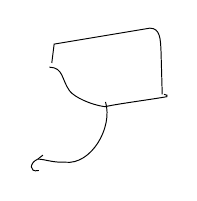
\begin{tikzpicture}[x=0.75cm,y=0.75cm]
\draw[line width=0.35pt] (0.12,-0.62) -- (0.16,-0.30) -- (1.78,-0.03)
  .. controls (1.96,-0.03) and (1.96,-0.22) .. (1.97,-0.43) -- (1.99,-1.15);
\draw[line width=0.35pt] (0.08,-0.69)
  .. controls (0.32,-0.70) and (0.28,-0.89) .. (0.42,-1.09)
  .. controls (0.50,-1.20) and (0.79,-1.33) .. (1.02,-1.36)
  .. controls (1.24,-1.31) and (1.79,-1.24) .. (2.07,-1.19)
  .. controls (2.10,-1.18) and (2.06,-1.15) .. (2.02,-1.15);
\draw[line width=0.35pt] (1.03,-1.28)
  .. controls (1.16,-1.72) and (0.78,-2.35) .. (0.35,-2.30)
  .. controls (0.12,-2.31) and (-0.02,-2.24) .. (-0.12,-2.25);
\draw[line width=0.35pt] (-0.12,-2.25)
  .. controls (-0.25,-2.30) and (-0.28,-2.48) .. (-0.10,-2.44);
\draw[line width=0.35pt] (-0.12,-2.25) -- (-0.03,-2.18);
\end{tikzpicture}}}

APPENDICE .- Ultraschémas et espaces algébriques de Serre\dotfill

App.1. Spectres maximaux et ultraschémas\dotfill

App.2. Espaces algébriques de Serre\dotfill

BIBLIOGRAPHIE\dotfill

INDEX DES NOTATIONS\dotfill

INDEX TERMINOLOGIQUE\dotfill

\begin{center}\rule{2cm}{0.4pt}\end{center}
% archive sheet number: 90
